
%% bare_jrnl_compsoc.tex
%% V1.3
%% 2007/01/11
%% by Michael Shell
%% See:
%% http://www.michaelshell.org/
%% for current contact information.
%%
%% This is a skeleton file demonstrating the use of IEEEtran.cls
%% (requires IEEEtran.cls version 1.7 or later) with an IEEE Computer
%% Society journal paper.
%%
%% Support sites:
%% http://www.michaelshell.org/tex/ieeetran/
%% http://www.ctan.org/tex-archive/macros/latex/contrib/IEEEtran/
%% and
%% http://www.ieee.org/

%%*************************************************************************
%% Legal Notice:
%% This code is offered as-is without any warranty either expressed or
%% implied; without even the implied warranty of MERCHANTABILITY or
%% FITNESS FOR A PARTICULAR PURPOSE! 
%% User assumes all risk.
%% In no event shall IEEE or any contributor to this code be liable for
%% any damages or losses, including, but not limited to, incidental,
%% consequential, or any other damages, resulting from the use or misuse
%% of any information contained here.
%%
%% All comments are the opinions of their respective authors and are not
%% necessarily endorsed by the IEEE.
%%
%% This work is distributed under the LaTeX Project Public License (LPPL)
%% ( http://www.latex-project.org/ ) version 1.3, and may be freely used,
%% distributed and modified. A copy of the LPPL, version 1.3, is included
%% in the base LaTeX documentation of all distributions of LaTeX released
%% 2003/12/01 or later.
%% Retain all contribution notices and credits.
%% ** Modified files should be clearly indicated as such, including  **
%% ** renaming them and changing author support contact information. **
%%
%% File list of work: IEEEtran.cls, IEEEtran_HOWTO.pdf, bare_adv.tex,
%%                    bare_conf.tex, bare_jrnl.tex, bare_jrnl_compsoc.tex
%%*************************************************************************

% *** Authors should verify (and, if needed, correct) their LaTeX system  ***
% *** with the testflow diagnostic prior to trusting their LaTeX platform ***
% *** with production work. IEEE's font choices can trigger bugs that do  ***
% *** not appear when using other class files.                            ***
% The testflow support page is at:
% http://www.michaelshell.org/tex/testflow/




% Note that the a4paper option is mainly intended so that authors in
% countries using A4 can easily print to A4 and see how their papers will
% look in print - the typesetting of the document will not typically be
% affected with changes in paper size (but the bottom and side margins will).
% Use the testflow package mentioned above to verify correct handling of
% both paper sizes by the user's LaTeX system.
%
% Also note that the "draftcls" or "draftclsnofoot", not "draft", option
% should be used if it is desired that the figures are to be displayed in
% draft mode.
%
% The Computer Society usually requires 12pt for submissions.
%
\documentclass[journal,compsoc]{../IEEE/IEEEtran}
%
% If IEEEtran.cls has not been installed into the LaTeX system files,
% manually specify the path to it like:
% \documentclass[12pt,journal,compsoc]{../sty/IEEEtran}





% Some very useful LaTeX packages include:
% (uncomment the ones you want to load)


% *** MISC UTILITY PACKAGES ***
%
%\usepackage{ifpdf}
% Heiko Oberdiek's ifpdf.sty is very useful if you need conditional
% compilation based on whether the output is pdf or dvi.
% usage:
% \ifpdf
%   % pdf code
% \else
%   % dvi code
% \fi
% The latest version of ifpdf.sty can be obtained from:
% http://www.ctan.org/tex-archive/macros/latex/contrib/oberdiek/
% Also, note that IEEEtran.cls V1.7 and later provides a builtin
% \ifCLASSINFOpdf conditional that works the same way.
% When switching from latex to pdflatex and vice-versa, the compiler may
% have to be run twice to clear warning/error messages.






% *** CITATION PACKAGES ***
%
\ifCLASSOPTIONcompsoc
  % IEEE Computer Society needs nocompress option
  % requires cite.sty v4.0 or later (November 2003)
  % \usepackage[nocompress]{cite}
\else
  % normal IEEE
  % \usepackage{cite}
\fi
% cite.sty was written by Donald Arseneau
% V1.6 and later of IEEEtran pre-defines the format of the cite.sty package
% \cite{} output to follow that of IEEE. Loading the cite package will
% result in citation numbers being automatically sorted and properly
% "compressed/ranged". e.g., [1], [9], [2], [7], [5], [6] without using
% cite.sty will become [1], [2], [5]--[7], [9] using cite.sty. cite.sty's
% \cite will automatically add leading space, if needed. Use cite.sty's
% noadjust option (cite.sty V3.8 and later) if you want to turn this off.
% cite.sty is already installed on most LaTeX systems. Be sure and use
% version 4.0 (2003-05-27) and later if using hyperref.sty. cite.sty does
% not currently provide for hyperlinked citations.
% The latest version can be obtained at:
% http://www.ctan.org/tex-archive/macros/latex/contrib/cite/
% The documentation is contained in the cite.sty file itself.
%
% Note that some packages require special options to format as the Computer
% Society requires. In particular, Computer Society  papers do not use
% compressed citation ranges as is done in typical IEEE papers
% (e.g., [1]-[4]). Instead, they list every citation separately in order
% (e.g., [1], [2], [3], [4]). To get the latter we need to load the cite
% package with the nocompress option which is supported by cite.sty v4.0
% and later. Note also the use of a CLASSOPTION conditional provided by
% IEEEtran.cls V1.7 and later.





% *** GRAPHICS RELATED PACKAGES ***
%
\ifCLASSINFOpdf
  % \usepackage[pdftex]{graphicx}
  % declare the path(s) where your graphic files are
  % \graphicspath{{../pdf/}{../jpeg/}}
  % and their extensions so you won't have to specify these with
  % every instance of \includegraphics
  % \DeclareGraphicsExtensions{.pdf,.jpeg,.png}
\else
  % or other class option (dvipsone, dvipdf, if not using dvips). graphicx
  % will default to the driver specified in the system graphics.cfg if no
  % driver is specified.
  % \usepackage[dvips]{graphicx}
  % declare the path(s) where your graphic files are
  % \graphicspath{{../eps/}}
  % and their extensions so you won't have to specify these with
  % every instance of \includegraphics
  % \DeclareGraphicsExtensions{.eps}
\fi
% graphicx was written by David Carlisle and Sebastian Rahtz. It is
% required if you want graphics, photos, etc. graphicx.sty is already
% installed on most LaTeX systems. The latest version and documentation can
% be obtained at: 
% http://www.ctan.org/tex-archive/macros/latex/required/graphics/
% Another good source of documentation is "Using Imported Graphics in
% LaTeX2e" by Keith Reckdahl which can be found as epslatex.ps or
% epslatex.pdf at: http://www.ctan.org/tex-archive/info/
%
% latex, and pdflatex in dvi mode, support graphics in encapsulated
% postscript (.eps) format. pdflatex in pdf mode supports graphics
% in .pdf, .jpeg, .png and .mps (metapost) formats. Users should ensure
% that all non-photo figures use a vector format (.eps, .pdf, .mps) and
% not a bitmapped formats (.jpeg, .png). IEEE frowns on bitmapped formats
% which can result in "jaggedy"/blurry rendering of lines and letters as
% well as large increases in file sizes.
%
% You can find documentation about the pdfTeX application at:
% http://www.tug.org/applications/pdftex





% *** MATH PACKAGES ***
%
%\usepackage[cmex10]{amsmath}
% A popular package from the American Mathematical Society that provides
% many useful and powerful commands for dealing with mathematics. If using
% it, be sure to load this package with the cmex10 option to ensure that
% only type 1 fonts will utilized at all point sizes. Without this option,
% it is possible that some math symbols, particularly those within
% footnotes, will be rendered in bitmap form which will result in a
% document that can not be IEEE Xplore compliant!
%
% Also, note that the amsmath package sets \interdisplaylinepenalty to 10000
% thus preventing page breaks from occurring within multiline equations. Use:
%\interdisplaylinepenalty=2500
% after loading amsmath to restore such page breaks as IEEEtran.cls normally
% does. amsmath.sty is already installed on most LaTeX systems. The latest
% version and documentation can be obtained at:
% http://www.ctan.org/tex-archive/macros/latex/required/amslatex/math/





% *** SPECIALIZED LIST PACKAGES ***
%
%\usepackage{algorithmic}
% algorithmic.sty was written by Peter Williams and Rogerio Brito.
% This package provides an algorithmic environment fo describing algorithms.
% You can use the algorithmic environment in-text or within a figure
% environment to provide for a floating algorithm. Do NOT use the algorithm
% floating environment provided by algorithm.sty (by the same authors) or
% algorithm2e.sty (by Christophe Fiorio) as IEEE does not use dedicated
% algorithm float types and packages that provide these will not provide
% correct IEEE style captions. The latest version and documentation of
% algorithmic.sty can be obtained at:
% http://www.ctan.org/tex-archive/macros/latex/contrib/algorithms/
% There is also a support site at:
% http://algorithms.berlios.de/index.html
% Also of interest may be the (relatively newer and more customizable)
% algorithmicx.sty package by Szasz Janos:
% http://www.ctan.org/tex-archive/macros/latex/contrib/algorithmicx/




% *** ALIGNMENT PACKAGES ***
%
%\usepackage{array}
% Frank Mittelbach's and David Carlisle's array.sty patches and improves
% the standard LaTeX2e array and tabular environments to provide better
% appearance and additional user controls. As the default LaTeX2e table
% generation code is lacking to the point of almost being broken with
% respect to the quality of the end results, all users are strongly
% advised to use an enhanced (at the very least that provided by array.sty)
% set of table tools. array.sty is already installed on most systems. The
% latest version and documentation can be obtained at:
% http://www.ctan.org/tex-archive/macros/latex/required/tools/


%\usepackage{mdwmath}
%\usepackage{mdwtab}
% Also highly recommended is Mark Wooding's extremely powerful MDW tools,
% especially mdwmath.sty and mdwtab.sty which are used to format equations
% and tables, respectively. The MDWtools set is already installed on most
% LaTeX systems. The lastest version and documentation is available at:
% http://www.ctan.org/tex-archive/macros/latex/contrib/mdwtools/


% IEEEtran contains the IEEEeqnarray family of commands that can be used to
% generate multiline equations as well as matrices, tables, etc., of high
% quality.


%\usepackage{eqparbox}
% Also of notable interest is Scott Pakin's eqparbox package for creating
% (automatically sized) equal width boxes - aka "natural width parboxes".
% Available at:
% http://www.ctan.org/tex-archive/macros/latex/contrib/eqparbox/





% *** SUBFIGURE PACKAGES ***
%\ifCLASSOPTIONcompsoc
%\usepackage[tight,normalsize,sf,SF]{subfigure}
%\else
%\usepackage[tight,footnotesize]{subfigure}
%\fi
% subfigure.sty was written by Steven Douglas Cochran. This package makes it
% easy to put subfigures in your figures. e.g., "Figure 1a and 1b". For IEEE
% work, it is a good idea to load it with the tight package option to reduce
% the amount of white space around the subfigures. Computer Society papers
% use a larger font and \sffamily font for their captions, hence the
% additional options needed under compsoc mode. subfigure.sty is already
% installed on most LaTeX systems. The latest version and documentation can
% be obtained at:
% http://www.ctan.org/tex-archive/obsolete/macros/latex/contrib/subfigure/
% subfigure.sty has been superceeded by subfig.sty.


%\ifCLASSOPTIONcompsoc
%  \usepackage[caption=false]{caption}
%  \usepackage[font=normalsize,labelfont=sf,textfont=sf]{subfig}
%\else
%  \usepackage[caption=false]{caption}
%  \usepackage[font=footnotesize]{subfig}
%\fi
% subfig.sty, also written by Steven Douglas Cochran, is the modern
% replacement for subfigure.sty. However, subfig.sty requires and
% automatically loads Axel Sommerfeldt's caption.sty which will override
% IEEEtran.cls handling of captions and this will result in nonIEEE style
% figure/table captions. To prevent this problem, be sure and preload
% caption.sty with its "caption=false" package option. This is will preserve
% IEEEtran.cls handing of captions. Version 1.3 (2005/06/28) and later 
% (recommended due to many improvements over 1.2) of subfig.sty supports
% the caption=false option directly:
%\ifCLASSOPTIONcompsoc
%  \usepackage[caption=false,font=normalsize,labelfont=sf,textfont=sf]{subfig}
%\else
%  \usepackage[caption=false,font=footnotesize]{subfig}
%\fi
%
% The latest version and documentation can be obtained at:
% http://www.ctan.org/tex-archive/macros/latex/contrib/subfig/
% The latest version and documentation of caption.sty can be obtained at:
% http://www.ctan.org/tex-archive/macros/latex/contrib/caption/




% *** FLOAT PACKAGES ***
%
%\usepackage{fixltx2e}
% fixltx2e, the successor to the earlier fix2col.sty, was written by
% Frank Mittelbach and David Carlisle. This package corrects a few problems
% in the LaTeX2e kernel, the most notable of which is that in current
% LaTeX2e releases, the ordering of single and double column floats is not
% guaranteed to be preserved. Thus, an unpatched LaTeX2e can allow a
% single column figure to be placed prior to an earlier double column
% figure. The latest version and documentation can be found at:
% http://www.ctan.org/tex-archive/macros/latex/base/



%\usepackage{stfloats}
% stfloats.sty was written by Sigitas Tolusis. This package gives LaTeX2e
% the ability to do double column floats at the bottom of the page as well
% as the top. (e.g., "\begin{figure*}[!b]" is not normally possible in
% LaTeX2e). It also provides a command:
%\fnbelowfloat
% to enable the placement of footnotes below bottom floats (the standard
% LaTeX2e kernel puts them above bottom floats). This is an invasive package
% which rewrites many portions of the LaTeX2e float routines. It may not work
% with other packages that modify the LaTeX2e float routines. The latest
% version and documentation can be obtained at:
% http://www.ctan.org/tex-archive/macros/latex/contrib/sttools/
% Documentation is contained in the stfloats.sty comments as well as in the
% presfull.pdf file. Do not use the stfloats baselinefloat ability as IEEE
% does not allow \baselineskip to stretch. Authors submitting work to the
% IEEE should note that IEEE rarely uses double column equations and
% that authors should try to avoid such use. Do not be tempted to use the
% cuted.sty or midfloat.sty packages (also by Sigitas Tolusis) as IEEE does
% not format its papers in such ways.




%\ifCLASSOPTIONcaptionsoff
%  \usepackage[nomarkers]{endfloat}
% \let\MYoriglatexcaption\caption
% \renewcommand{\caption}[2][\relax]{\MYoriglatexcaption[#2]{#2}}
%\fi
% endfloat.sty was written by James Darrell McCauley and Jeff Goldberg.
% This package may be useful when used in conjunction with IEEEtran.cls'
% captionsoff option. Some IEEE journals/societies require that submissions
% have lists of figures/tables at the end of the paper and that
% figures/tables without any captions are placed on a page by themselves at
% the end of the document. If needed, the draftcls IEEEtran class option or
% \CLASSINPUTbaselinestretch interface can be used to increase the line
% spacing as well. Be sure and use the nomarkers option of endfloat to
% prevent endfloat from "marking" where the figures would have been placed
% in the text. The two hack lines of code above are a slight modification of
% that suggested by in the endfloat docs (section 8.3.1) to ensure that
% the full captions always appear in the list of figures/tables - even if
% the user used the short optional argument of \caption[]{}.
% IEEE papers do not typically make use of \caption[]'s optional argument,
% so this should not be an issue. A similar trick can be used to disable
% captions of packages such as subfig.sty that lack options to turn off
% the subcaptions:
% For subfig.sty:
% \let\MYorigsubfloat\subfloat
% \renewcommand{\subfloat}[2][\relax]{\MYorigsubfloat[]{#2}}
% For subfigure.sty:
% \let\MYorigsubfigure\subfigure
% \renewcommand{\subfigure}[2][\relax]{\MYorigsubfigure[]{#2}}
% However, the above trick will not work if both optional arguments of
% the \subfloat/subfig command are used. Furthermore, there needs to be a
% description of each subfigure *somewhere* and endfloat does not add
% subfigure captions to its list of figures. Thus, the best approach is to
% avoid the use of subfigure captions (many IEEE journals avoid them anyway)
% and instead reference/explain all the subfigures within the main caption.
% The latest version of endfloat.sty and its documentation can obtained at:
% http://www.ctan.org/tex-archive/macros/latex/contrib/endfloat/
%
% The IEEEtran \ifCLASSOPTIONcaptionsoff conditional can also be used
% later in the document, say, to conditionally put the References on a 
% page by themselves.




% *** PDF, URL AND HYPERLINK PACKAGES ***
%
%\usepackage{url}
% url.sty was written by Donald Arseneau. It provides better support for
% handling and breaking URLs. url.sty is already installed on most LaTeX
% systems. The latest version can be obtained at:
% http://www.ctan.org/tex-archive/macros/latex/contrib/misc/
% Read the url.sty source comments for usage information. Basically,
% \url{my_url_here}.





% *** Do not adjust lengths that control margins, column widths, etc. ***
% *** Do not use packages that alter fonts (such as pslatex).         ***
% There should be no need to do such things with IEEEtran.cls V1.6 and later.
% (Unless specifically asked to do so by the journal or conference you plan
% to submit to, of course. )






\usepackage[utf8x]{inputenc}
\usepackage{todonotes}
\usepackage{hyperref}
\usepackage{cleveref}
\usepackage[cmex10]{amsmath}
\usepackage{algpseudocode}
%\usepackage{algorithmicx}
\usepackage{algorithm}

\usepackage{graphicx}
% declare the path(s) where your graphic files are
\graphicspath{{images/}}
\usepackage{caption}
\usepackage{subcaption}

\usepackage{xspace}
\newcommand{\computeflux}{\texttt{compute\_flux}\xspace}
\newcommand{\update}{\texttt{update}\xspace}
\newcommand{\polu}{\texttt{polu}\xspace}
\newcommand{\dirichlet}{\textit{Dirichlet}\xspace}





% correct bad hyphenation here
\hyphenation{op-tical net-works semi-conduc-tor}


\begin{document}
%
% paper title
% can use linebreaks \\ within to get better formatting as desired
\title{A Finite Volume Case Study From An Industrial Application}
%
%
% author names and IEEE memberships
% note positions of commas and nonbreaking spaces ( ~ ) LaTeX will not break
% a structure at a ~ so this keeps an author's name from being broken across
% two lines.
% use \thanks{} to gain access to the first footnote area
% a separate \thanks must be used for each paragraph as LaTeX2e's \thanks
% was not built to handle multiple paragraphs
%
%
%\IEEEcompsocitemizethanks is a special \thanks that produces the bulleted
% lists the Computer Society journals use for "first footnote" author
% affiliations. Use \IEEEcompsocthanksitem which works much like \item
% for each affiliation group. When not in compsoc mode,
% \IEEEcompsocitemizethanks becomes like \thanks and
% \IEEEcompsocthanksitem becomes a line break with idention. This
% facilitates dual compilation, although admittedly the differences in the
% desired content of \author between the different types of papers makes a
% one-size-fits-all approach a daunting prospect. For instance, compsoc 
% journal papers have the author affiliations above the "Manuscript
% received ..."  text while in non-compsoc journals this is reversed. Sigh.

\author{Miguel~Palhas,~\IEEEmembership{pg19808,~MEI}
        , Pedro~Costa,~\IEEEmembership{pg19830,~MEI}
        and Stéphane~Clain,~\IEEEmembership{co-Advisor}%
  \IEEEcompsocitemizethanks{%
    \IEEEcompsocthanksitem{M. Palhas and P. Costa are with the Department of Informatics at University of Minho, Braga, Portugal\protect\\%
      E-mail: \texttt{pg\{19808,19830\}@alunos.uminho.pt}
    }
    \IEEEcompsocthanksitem{Professor Doctor Stéphane Clain is with the Department of Mathematics and Applications at University of Minho, Braga, Portugal\protect\\%
      E-mail: \texttt{clain@math.uminho.pt}
    }
  }
}


% \author{Michael~Shell,~\IEEEmembership{Member,~IEEE,}
%         John~Doe,~\IEEEmembership{Fellow,~OSA,}
%         and~Jane~Doe,~\IEEEmembership{Life~Fellow,~IEEE}% <-this % stops a space
% \IEEEcompsocitemizethanks{\IEEEcompsocthanksitem M. Shell is with the Department
% of Electrical and Computer Engineering, Georgia Institute of Technology, Atlanta,
% GA, 30332.\protect\\
% % note need leading \protect in front of \\ to get a newline within \thanks as
% % \\ is fragile and will error, could use \hfil\break instead.
% E-mail: see http://www.michaelshell.org/contact.html
% \IEEEcompsocthanksitem J. Doe and J. Doe are with Anonymous University.}% <-this % stops a space
% \thanks{Manuscript received April 19, 2005; revised January 11, 2007.}}

% note the % following the last \IEEEmembership and also \thanks - 
% these prevent an unwanted space from occurring between the last author name
% and the end of the author line. i.e., if you had this:
% 
% \author{....lastname \thanks{...} \thanks{...} }
%                     ^------------^------------^----Do not want these spaces!
%
% a space would be appended to the last name and could cause every name on that
% line to be shifted left slightly. This is one of those "LaTeX things". For
% instance, "\textbf{A} \textbf{B}" will typeset as "A B" not "AB". To get
% "AB" then you have to do: "\textbf{A}\textbf{B}"
% \thanks is no different in this regard, so shield the last } of each \thanks
% that ends a line with a % and do not let a space in before the next \thanks.
% Spaces after \IEEEmembership other than the last one are OK (and needed) as
% you are supposed to have spaces between the names. For what it is worth,
% this is a minor point as most people would not even notice if the said evil
% space somehow managed to creep in.



% The paper headers
\markboth{Integrated Project, Parallel and Distributed Computing, June~2012}%
{Palhas and Costa: A Finite Volume Case Study From An Industrial Application}
% The only time the second header will appear is for the odd numbered pages
% after the title page when using the twoside option.
% 
% *** Note that you probably will NOT want to include the author's ***
% *** name in the headers of peer review papers.                   ***
% You can use \ifCLASSOPTIONpeerreview for conditional compilation here if
% you desire.



% The publisher's ID mark at the bottom of the page is less important with
% Computer Society journal papers as those publications place the marks
% outside of the main text columns and, therefore, unlike regular IEEE
% journals, the available text space is not reduced by their presence.
% If you want to put a publisher's ID mark on the page you can do it like
% this:
%\IEEEpubid{0000--0000/00\$00.00~\copyright~2007 IEEE}
% or like this to get the Computer Society new two part style.
%\IEEEpubid{\makebox[\columnwidth]{\hfill 0000--0000/00/\$00.00~\copyright~2007 IEEE}%
%\hspace{\columnsep}\makebox[\columnwidth]{Published by the IEEE Computer Society\hfill}}
% Remember, if you use this you must call \IEEEpubidadjcol in the second
% column for its text to clear the IEEEpubid mark (Computer Society jorunal
% papers don't need this extra clearance.)



% use for special paper notices
%\IEEEspecialpapernotice{(Invited Paper)}



% for Computer Society papers, we must declare the abstract and index terms
% PRIOR to the title within the \IEEEcompsoctitleabstractindextext IEEEtran
% command as these need to go into the title area created by \maketitle.
\IEEEcompsoctitleabstractindextext{%
\begin{abstract}
%\boldmath
\todo[inline]{This template is quite acceptable for a paper, but IMO it is unfit for a technical/scientific report for a class}
\todo[inline]{When the first cite is placed, replace the bibliography with the proper mechanism}


\end{abstract}
% IEEEtran.cls defaults to using nonbold math in the Abstract.
% This preserves the distinction between vectors and scalars. However,
% if the journal you are submitting to favors bold math in the abstract,
% then you can use LaTeX's standard command \boldmath at the very start
% of the abstract to achieve this. Many IEEE journals frown on math
% in the abstract anyway. In particular, the Computer Society does
% not want either math or citations to appear in the abstract.

% Note that keywords are not normally used for peerreview papers.
\begin{IEEEkeywords}
Computer Society, IEEEtran, journal, \LaTeX, paper, template.
\end{IEEEkeywords}}


% make the title area
\maketitle


% To allow for easy dual compilation without having to reenter the
% abstract/keywords data, the \IEEEcompsoctitleabstractindextext text will
% not be used in maketitle, but will appear (i.e., to be "transported")
% here as \IEEEdisplaynotcompsoctitleabstractindextext when compsoc mode
% is not selected <OR> if conference mode is selected - because compsoc
% conference papers position the abstract like regular (non-compsoc)
% papers do!
\IEEEdisplaynotcompsoctitleabstractindextext
% \IEEEdisplaynotcompsoctitleabstractindextext has no effect when using
% compsoc under a non-conference mode.


% For peer review papers, you can put extra information on the cover
% page as needed:
% \ifCLASSOPTIONpeerreview
% \begin{center} \bfseries EDICS Category: 3-BBND \end{center}
% \fi
%
% For peerreview papers, this IEEEtran command inserts a page break and
% creates the second title. It will be ignored for other modes.
\IEEEpeerreviewmaketitle



% \section{Introduction}
% Computer Society journal papers do something a tad strange with the very
% first section heading (almost always called "Introduction"). They place it
% ABOVE the main text! IEEEtran.cls currently does not do this for you.
% However, You can achieve this effect by making LaTeX jump through some
% hoops via something like:
%
%\ifCLASSOPTIONcompsoc
%  \noindent\raisebox{2\baselineskip}[0pt][0pt]%
%  {\parbox{\columnwidth}{\section{Introduction}\label{sec:introduction}%
%  \global\everypar=\everypar}}%
%  \vspace{-1\baselineskip}\vspace{-\parskip}\par
%\else
%  \section{Introduction}\label{sec:introduction}\par
%\fi
%
% Admittedly, this is a hack and may well be fragile, but seems to do the
% trick for me. Note the need to keep any \label that may be used right
% after \section in the above as the hack puts \section within a raised box.



% The very first letter is a 2 line initial drop letter followed
% by the rest of the first word in caps (small caps for compsoc).
% 
% form to use if the first word consists of a single letter:
% \IEEEPARstart{A}{demo} file is ....
% 
% form to use if you need the single drop letter followed by
% normal text (unknown if ever used by IEEE):
% \IEEEPARstart{A}{}demo file is ....
% 
% Some journals put the first two words in caps:
% \IEEEPARstart{T}{his demo} file is ....
% 
% Here we have the typical use of a "T" for an initial drop letter
% and "HIS" in caps to complete the first word.
% \IEEEPARstart{T}{his} demo file is intended to serve as a ``starter file''
% for IEEE Computer Society journal papers produced under \LaTeX\ using
% IEEEtran.cls version 1.7 and later.
% % You must have at least 2 lines in the paragraph with the drop letter
% % (should never be an issue)
% I wish you the best of success.

% \hfill mds
 
% \hfill January 11, 2007

% \subsection{Subsection Heading Here}
% Subsection text here.

% % needed in second column of first page if using \IEEEpubid
% %\IEEEpubidadjcol

% \subsubsection{Subsubsection Heading Here}
% Subsubsection text here.

\section{Introduction}
\label{sec:intro}

This document describes an incremental work where the \texttt{polu} application, which computes the propagation of a pollutant in a two dimensional environment, was studied in order to find possibilities of optimization and/or parallelization.

The \texttt{polu} application is built on top of the Finite Volume Library (FVL) which is also a focus of study in this document, as a large part of the logic and data structures are implemented on it, rather than on the application itself. In this context, both of them are considered as a whole case study.

Several changes were performed in the original code, which are fully described in this document. Those changes vary in nature, from simple or low-level code optimization, to higher-level algorithmic changes, in order to allow parallelization and/or improve performance. The data structures used also suffered large changes (originally implemented as \textit{Arrays-of-Pointers}) to \textit{Arrays-of-Structures} at first, and also to \textit{Structure-of-Arrays}. This changes removed excessive dereferencing caused by deep chains of pointers in the original strucutres, effectively reducing memory accesses and improving locality.

The several phases that composed this project reflect on the multiple approaches and variety of results presented here. In general, the goal is to study the performance impact, advantages and difficulties of different programming paradigms, applied to the \texttt{polu} application. 


\todo[inline]{O paragrafo aqui a explicar o que é falado no relatorio}

After the initial analysis of initial sequential code, a shared-memory parallel implementation, using OpenMP \todo{ref sec:omp}, a distributed-memory implementation, with the \textit{Message Passing Interface} (MPI) \todo{ref sec:mpi}, and a GPU implementation (using CUDA) \todo{ref sec:cuda} were implemented and profiled.

\section{Case Study}
\todo[inline]{Explain what the program is meant for}

The application analyzed in this document computes, called here \texttt{polu}, computes the flux of a material (e.g. a pollutant) through a bidimensional surface. This surface is described as a mesh, composed mainly of edges and cells. The input is given by a 

The original \texttt{polu} application works like a heartbeat algorithm with no communication (since it is executed in a single computation node). The algorithm used by the application sees the environment as a discrete mesh (represented by its cells and edges) and loops until the specified time interval is reached. At each iteration of this main loop, the algorithm performs two main steps:

\begin{description}[\IEEEsetlabelwidth{Pollution Update}\IEEEusemathlabelsep]
	\item[Flux Computation] Based on current pollution values for each cell, the flux for each edge is calculated (performed by the \texttt{compute\_flux} function)
	\item[Pollution Update] Using the previously calculated flux values, the pollution for each cell is updated (performed by the \texttt{update} function)
\end{description}

\subsection{Algorithm}

The algorithm used by the \polu application is a first order finite volume method. This means that each mesh element only communicates directly with its first level neighbors in the mesh, which makes this a typical case of a stencil computation. In terms of performance, being a stencil algorithm implies that the operational intensity \todo[inline]{ref ao paper do roofline} will most likely remain constant with larger problem sizes. On the other hand, the low order allows for a greater locality of the calculations, and favors parallelization.

The code consists on a preparation stage, where all the required elements are loaded and prepared, and two computation stages, which compose the main loop.

Operations performed in the preparation stage are highly dependent on the implementation being described, as most will require some elements to be properly organized or some values to be previously computed. Common operations, such as loading the necessary data from the described files are constant to every implementation, but may still differ in the structures used to store the data.

A single execution of the two computation stages together form a step in the iterative method behind this application. These stages, also referred in this document as core functions, or kernels, are the \computeflux and \update functions.

In \computeflux, all the edges in the mesh are analyzed, and the flux of pollution to be transfered across that edge is computed, based on the polution level and the velocity vectors of the cells it connects. A preconfigured value is used as the \dirichlet condition\footnote{The \dirichlet condition is a type of boundary condition used to specify a value taken by the solution in the border of the domain. In the \polu application, this value is constant throughout the execution}, which replaces the polution level of a second cell for the edges in the border of the mesh.

As for the \update function, it uses the computed flux values to update the polution levels of each cell in the mesh, by adding the individual contribution of each edge of the cell. While triangular cells are prefered, there are no restrictions to the number of edges a cell may have.

\subsection{Parallelism Oportunities}
\todo[inline]{Explain what can be executed in parallel}
\todo[inline]{Mention this is a heartbeat}

During the main loop of this program both core functions, \computeflux and \update, depend on each other to perform their tasks. \update requires flux from all edges to be previously computed in \computeflux, which in turn requires that all pollution values are up-to-date to correctly compute the flux for the next iteration. This creates two implicit synchronization points in the main loop, and is a consequence of the heartbeat characteristics of the problem.

This allows both functions to be looked at as individual tasks, that may be subject to different parallelization approaches. Both functions perform calculations using the entire mesh, but they differ in the element used: while \computeflux iterates over edges, \update iterates over cells.

\todo[inline,color=green!40]{Ainda tentei acabar eu isto mas não sei bem onde querias ir com este texto, por isso acaba tu. Pode ser útil um parágrafo a explicar que nos algoritmos de stencil é comum deixar-se que diferentes partes da mesh estejam em diferentes iterações por só terem dependência local, mas que no nosso caso por ser um heartbeat isto não é de todo trivial de implementar.}

\section{Sequential}
\label{sec:seq}

\todorev{Written on Sat, June 30 at 13:16 by pfac}

In this section are presented the sequential implementations of \polu, from the original to the optimized versions. \Cref{sec:seq:limitations} analyzes the dependencies in the sequential code which prevent the parallelization of the core functions (as explained in \cref{sec:220}), and how the code was adapted to remove them. 

\subsection{Original}
\label{sec:310}
%\todo[inline,color=blue!40]{Add some algebra to the core functions text. Hard to keep track with only text.}

The original \polu program was implemented using structures as \textit{Arrays-Of-Pointers} (AOP). While this allows for an easier development and better code readability, the deep levels of dereferencing imply an increased number of memory accesses, which aggravate the effects of any memory bottlenecks.

In this original version, the \computeflux function iterates over each edge, and loads the pollution levels and velocity vectors of the cells it connects. For edges in the border of the mesh, a convention is followed, indicating that the non existing cell is alwasy the right one (cells are refered to as left and right cells of a given edge). When the right cell doesn't exist, the \dirichlet condition is used as the value for that border.

The velocity vector in the edge is computed based on the velocity of both cells and the normal of the edge. This final velocity also gives information about the direction of the flux. A positive velocity makes the pollution flow from left to right, and the inverse happens with a negative velocity. \Cref{alg:flux} illustrates this behavious.



\begin{figure}[!htp]
	\begin{alg}
		\ForAll {$edge \in Edges$}				\\
			$l     \gets left\_cells_{edge}$ 	\\
			$r     \gets rigth\_cells_{edge}$ 	\\
			$u_{l} \gets pollution_{l}$ 		
			\If {$\exists Cells_{r}$} 			\\
				$u_{r} \gets pollution_{r}$
			\Else 								\\
				$u_{r} \gets \dirichlet$ 
			\EndIf 	 							\\
			$v_{edge} \gets (v_{l} + v_{r}) / 2 \cdot normal_{edge}$ 					\\
			$v_{max} \gets max(v_{max}, v_{edge})$ 										\\
			$flux_{edge} += u_{l} \cdot [v_{edge}]^{+} + u_{r} \cdot [v_{edge}]^{-}$
		\EndFor
	\end{alg}

	\caption{Pseudocode for the original \computeflux function}
	\label{alg:flux}
\end{figure}

This function also returns the elapsed time, which is computed with the maximum absolute value of the computed edge velocities, and is used at the end of the iteration to keep track of the total elapsed time.

The original \update function also iterates over each edge. The contribution of each edge to the cells final value is computed as the product between the elapsed time, the computed flux and the ratio between the edge's length and the cell's area. This is described in \cref{alg:update}.

\begin{figure}[!htp]
	\begin{alg}
		\ForAll {$edge \in Edges$}

			$\Delta{u} \gets \Delta{t} \cdot flux_{edge} \cdot L_{edge}$

			$l \gets left\_cells_{edge}$

			$r \gets right\_cells_{edge}$

			$pollution_{l} -= \frac{\Delta{u}}{A_{l}}$

			\If {$\exists Cells_{r}$}

				$pollution_{r} \gets \frac{\Delta{u}}{A_{r}}$
			\EndIf
		\EndFor
	\end{alg}

	\caption{Original \update function}
	\label{alg:update}
\end{figure}



There is also the possibility to output the current state of the mesh after every $X$ of iterations, where $X$ is a parameter provided at runtime. This feature allows the output to contain not only the final state of the system byt all the intermediary states, allowing  an animation to be shown using \texttt{gmsh}.

\subsubsection{Simplifications}
% \todo[inline]{Animation and velocity calculation are out}

Two important simplifications were initially performed in the original version, before any other adaptation or rewrite of the code.

The first simplification meant removing the output operation at the end of each main loop iteration, thus removing the animation feature. While this feature is interesting to analyze how the system evolved, input/output operations are very slow when compared to computation operations. Since the main goal of this document is to study ways to improve the performance of the \polu application, this feature may be discarded.

The second major simplification focus on the \computeflux function. Since the every cell's velocity vector remains constant throughout the entire program's execution, the same values will be computed for the velocity in each edge and for the elapsed time. While this computation is important in a more dynamic application where velocity vectors are also updated, such is not the case for this algorithm. Therefore, it is possible to remove these two computational steps from the core function to the preprocessing stage, thus globally improving the program's performance.

\subsection{Optimizations}
\label{sec:seq:optimizations}

\todorev{Last revised on Sat, June 30 at 15:33 by pfac}

While optimizing the sequential code may be important to eliminate possible bottlenecks created by inefficient memory access patterns or poorly written code, most of the optimization work was kept for after the parallelization, as early optimizations might have hampered parallel implementations.
As such, the focus of optimization in the sequential implementation of \polu was on the structures used, which were trivially found to be very inefficient.

As previously stated, the original implementation relied on an AOP approach, but the excessively deep chains of pointers translate into more memory accesses, and consecutively worse performance.

The next two sections describe the two alternative approaches and explain how these improved the application's performance.

\subsubsection{AOS}
% \todo[inline]{Explain the AOS structures and why they should be better than AOP}

The first implemented alternative to AOP was the \textit{Arrays-Of-Structs} approach. Instead of using pointers, structures were created for cells and edges, containing all the data about each. Where pointers existed to link an edge to the adjacent cells, or a cell to its edges, an index is placed. While the dereferencing levels are completely eliminated, using indexes allows any element to hold identifiers which allows direct access to the other elements it needs to interact with, as long as all the data objects are stored in arrays. The maximum representable index is used as the equivalent to \texttt{NULL} pointers (applied, for example, to the right cell of a border edge).
\subsubsection{SOA}
% \todo[inline]{Explain the SOA structures and why they should be better than SOA}

While the AOS approach completely removes the need for dereference, using a \textit{Struct-Of-Arrays} (SOA) approach can be more efficient.

One of the problems with the AOS approach is that when the core functions iterate over one of the arrays, cache lines are being filled with the complete structure of these elements. Yet, neither of the core functions utilizes all the data in that structure, which translates in useless data occupying the cache. This hurts spatial locality\footnote{If a data element is required, it is highly probable adjacent elements will also be required in the near future.}, greatly increasing the chances of accessing a mesh element translating into a RAM access.

The SOA approach solves this problem by placing the data of each element in distinct. As an example, a single array is created to hold the polution level of all the cells. Each data piece is placed in a different array.

This approach allows the core functions to load only the data required for their compuations. The cache lines are now filled only with useful data, and the pieces which are required by the other functions will only be loaded when needed.
\subsubsection{Results}

\todorev{Written on Sat, June 30 at 21:40 by pfac}

To evaluate the impact of the optimizations presented in \cref{sec:321,sec:322}, performance tests were performed with the original and optimized versions.
\Cref{sec:env,sec:method} describe the environmental setup and methodology for the tests performed, respectively.

\Cref{fig:seq:results} shows the results obtained for the three sequential versions.
Both optimized versions show a clear improvement just by not using the several dereference levels. Also, the results show a clear improvement by using SOA over AOS, proving the effectiveness of the optimization.

\begin{figure}[!htp]
	\centering
	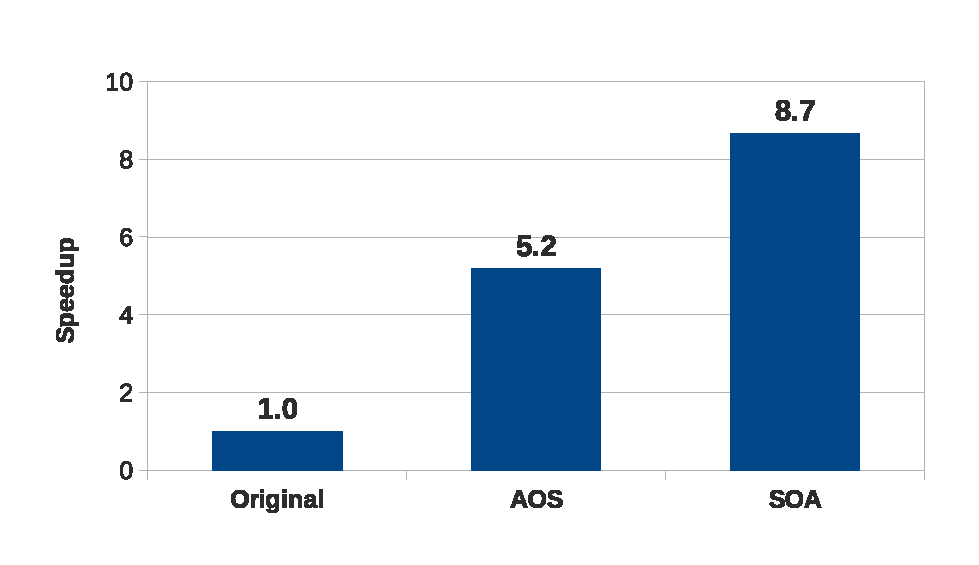
\includegraphics[width=\columnwidth]{images/graph_comparison_seq.eps}
	\caption{Speedup results for the three sequential versions, compared with the original version.}
	\label{fig:seq:results}
\end{figure}
\subsection{Limitations}

The main limitation for the sequential versions is the locality of the mesh used in the problem. Since this issue will be present in any shared memory implementation too, that discussion is left for \cref{sec:omp:limitations}.

\Cref{fig:roofline} shows the roofine for SeARCH Group 201 with the computational intensities of the SOA and AOS versions. Computational intensity is defined to be the ratio between all the instructions not related with memory accesses (loads and stores) and the number of bytes accessed in RAM.

The improvement from AOS to SOA can be explained only by the improvements in locality. Further testing, which results were omitted in this document, shown that the number of bytes acessed to RAM, number of computational instructions completed and the core functions execution time all decreased, achieving almost the same amount of computational instructions per second, while halving the number of accesses.

\begin{figure}
	\centering
	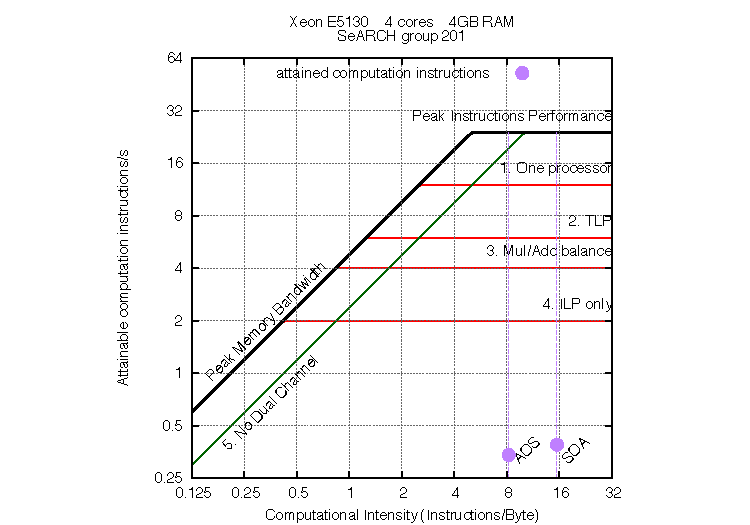
\includegraphics[width=\columnwidth]{images/roofline201m.pdf}
	\caption{Roofline for SeARCH Group 201, with the computational intensities of the AOS and SOA versions.}
	\label{fig:roofline201}
\end{figure}

\subsection{Dependencies}
\label{sec:dependencies}

\todorev{Last revised on Sat, June 30 at 21:47 by pfac}

\todoextra{Maybe add here a footnote to explain reductions.} 

As explained in \cref{sec:220}, the heartbeat nature of the algorithm prevents extending parallelization beyond the scope of each core function, but both functions are able to execute their internal iterations in parallel.
Yet, some dependencies exist among the elements used in these functions, and adaptations are required to allow parallelization.

\computeflux has only one dependency, in the computation of the elapsed time $\Delta t$, which is removed simply by accepting the second simplification described in \cref{sec:311}.
While this simplification is assumed in the final implementations, this dependency was properly studied in early stages of the project.
Since the computation of $\Delta t$ is based in a maximum operation, it is possible to replace this dependency with a reduction after the computation of the fluxes, thus removing the dependency and maintaining the correctness of the program.

On the other hand, the \update function has a dependency which may not be neglected because of a simplification.
As described in \cref{sec:310}, the original implementation of \update iterates over the edges.
While this may favor locality after executing \computeflux, it creates a race condition when each edges adds its own contribution to the cell's value.
This dependency can be removed by changing how \update iterates over the mesh. By iterating over the cells instead of the edges, the race condition disappears since only one write operation per cell is performed, as shown in \cref{alg:update}.

\begin{figure}[!htp]
	\begin{alg}
		\ForAll {$cell \in Cells$}
			\ForAll {$edge \in Edges_{cell}$}
				\State $pollution_{cell} += \Delta{t} \times flux_{edge} \times \frac{L_{edge}}{A_{cell}}$
			\EndFor
		\EndFor
	\end{alg}

	\caption{New \update function, now iterating over cells instead of edges}
	\label{alg:update2}
\end{figure}

<<<<<<< HEAD
\section{Shared Memory}

A shared memory parallel version of \polu was implemented using the OpenMP interface. The main feature about this API is that the program itself remains almost equal to the sequential version, requiring only the addition of the necessary directives and the adaptation of the code to remove dependencies.

Both core functions were parallelized adding a \texttt{parallel for} directive to the internal loops. The number of threads issued in each parallel zone is given as the second argument of the program, and defaults to the maximum number of threads supported by the hardware in the absence of the argument.

	\subsection{Load Balance}
% \todo[inline]{Describe the static scheduling with OpenMP and explain that all the iterations make the same operations in every function}

Both core functions are mostly homogeneous in its parallel implementation. In \computeflux, the two branches perform the same amount of operations whether they are followed or not. In \update, the heaviest part of the workload is constant (products and divisions), and it only differs in the number of edges contributing to the edge. While this value may cause the function to become heterogeneous, this is highly dependent on the mesh used (the test case used in \cref{sec:700} has 3 edges in every cell).

By default, the OpenMP interface uses static scheduling, where iterations are assigned to threads in a \textit{round-robin} pattern. Since the number of edges and cells is a constant throughout the entire execution, this guarantees the best load balancing among threads.

\subsection{Limitations}
% \todo[inline]{Describe the locality problems}
% \todo[inline]{Opportunity to show here that cute image that displays locality of the mesh}

The main problem with this implemetation is data locality. While these issues are softened using a SOA approach, and the method is a first order one, the algorithm is still not very cache friendly in either of the core functions.

In \computeflux, each edge requires access to data from the two adjacent cells. While the access to edges is contiguous, access to cells is not for most of the iterations. Yet, border edges do not require the second edge.

\update on the other hand requires access to all the edges in a cell, which are always more than two. Analogously, the access to cells is contiguous, but the access to edges is not. Since each edge has more edges, than an edge has adjacent cells, and since no edge may be neglect for any cell, this function is most likely the bottleneck of the main loop.
\section{Distributed Memory}
\label{sec:dist}

For a distributed memory implementation, and with the sequential code having already suffered some changes and optimizations

\todo[inline,color=green!40]{Describe the MPI implementation}

\subsection{Load Balance}
\label{subsec:dist:load}

\todo[inline,color=green!40]{Describe how the mesh was partitioned}

\subsection{Limitations}
\label{subsec:dist:limitations}
\todo[inline,color=green!40]{Explain how communication may be a problem, despite of locality issues being favored (smaller pieces of mesh)}




\section{GPU}
\todo[inline,color=green!40]{Describe the CUDA implementation}
\subsection{Load Balance}
\todo[inline,color=green!40]{Explain how the workload is assigned to each thread}
\subsection{Optimizations}
\todo[inline,color=green!40]{Explain source code optimizations, and their impact on performace}
\todo[inline,color=green!40]{Explain how the branches are simple but may still cause warps to diverge and whatever more}
\subsection{Mesh ordering impact}
\todo[inline,color=green!40]{Explain how better ordering of cells/edges should, theoretically, be useful to increase coalesced memory accesses}
\todo[inline,color=green!40]{Talk about the simple optimization attempt (mesh reorder) and its poor (maybe null?) impact on performance}
=======

\section{Shared Memory}
\todo[inline]{Describe the OpenMP implementations}
\subsection{Load Balance}
\todo[inline]{Describe the static scheduling with OpenMP and explain that all the iterations make the same operations in every function}
\subsection{Limitations}
\todo[inline]{Describe the locality problems}
\todo[inline]{Opportunity to show here that cute image that displays locality of the mesh}

\section{Distributed Memory}
\label{sec:mpi}

For a distributed memory implementation, The \textit{Message Passing Interface} (MPI) was used. With the sequential code having already suffered some changes and optimizations, the main problem consisted in the partitioning of the mesh. The obvious approach is one where each processor is assigned to a subset of the entire mesh, and is responsible for the application of both kernels to its subset. Communication is also required between each main loop iteration, since each process will require access to the values in the border of its subset, in order to compute its own values.

\subsection{Mesh Partitioning}
\label{subsec:mpi:partitioning}

In order to distribute processing payload across each process, the input mesh, and all of the data associated with it, also needs to be split into partitions. A mesh partitioning algorithm is required. This algorithm must generate $P$ disjoined partitions (where $P$ is the number of processors available), each to be assigned to a different processor. Some additional data is also required for each partition, so that information about how each partition connects to the others is kept, to allow communication to be done correctly.

\subsubsection{Research in Mesh Partitioning}
\label{subsubsec:mpi:partitioning:research}

Mesh partitioning is currently an actively researched topic, with some projects and libraries begin already available that help with the understanding of how a mesh (or more generically, a graph) can be partitioned in ways to optimize certain aspects like load balancing, communication balancing or partitioning overhead. For instance, in \cite{metis}, a library called \texttt{Metis} is presented whose purpose is precisely this problem. Other works found for this topic included \cite{gilbert1995, walshaw2000}.

However, given the time constraints of this project, and since the priority was to have a functional algorithm rather than an optimal one, it was decided not to attempt an approach involving \texttt{Metis} or any other researched work. Actually, the method used to partition the mesh is quite naive, as shown in \cref{subsubsec:mpi:partitioning:method}.

\subsubsection{Partitioning Methodology}
\label{subsubsec:mpi:partitioning:method}

he algorithm created to partition the mesh works by dividing it in slices by the horizontal coordinate of each cell. Givem a mesh with a total of 100 cells, and a pool of $P$ processes, the mesh is divided into $P$ partitions, each with exactly $N=100/P$ cells, differing by at most one cell when they cannot be evenly divided. By ordering the cells based on their $x$ coordinate, they are sequentially assigned to each process, in such a way that the first process receives the first $N$ cells of the set, and so on.

\begin{figure}[!htp]
	\begin{subfigure}[b]{0.5\columnwidth}
		\centering
		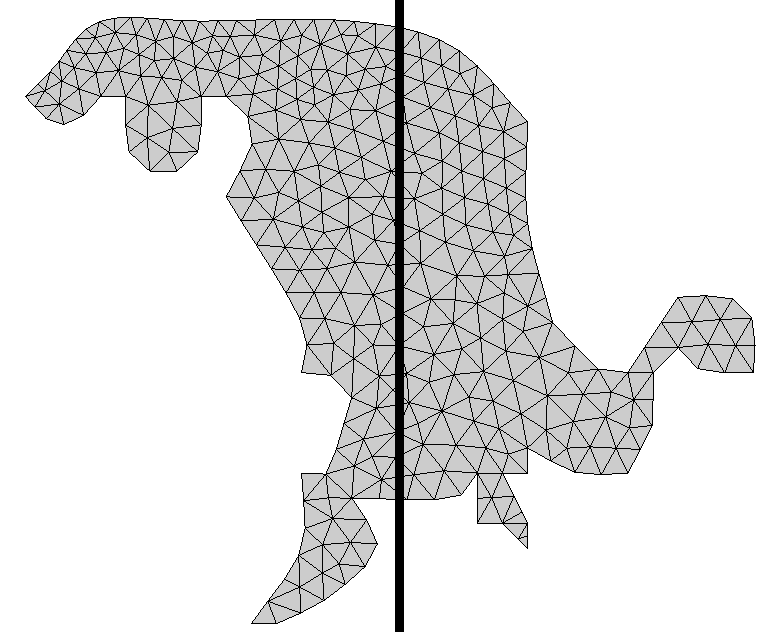
\includegraphics[width=\columnwidth]{foz_p2_msh}
		\caption{2 partitions}
		\label{fig:foz_p2_msh}
	\end{subfigure}%
	\begin{subfigure}[b]{0.5\columnwidth}
		\centering
		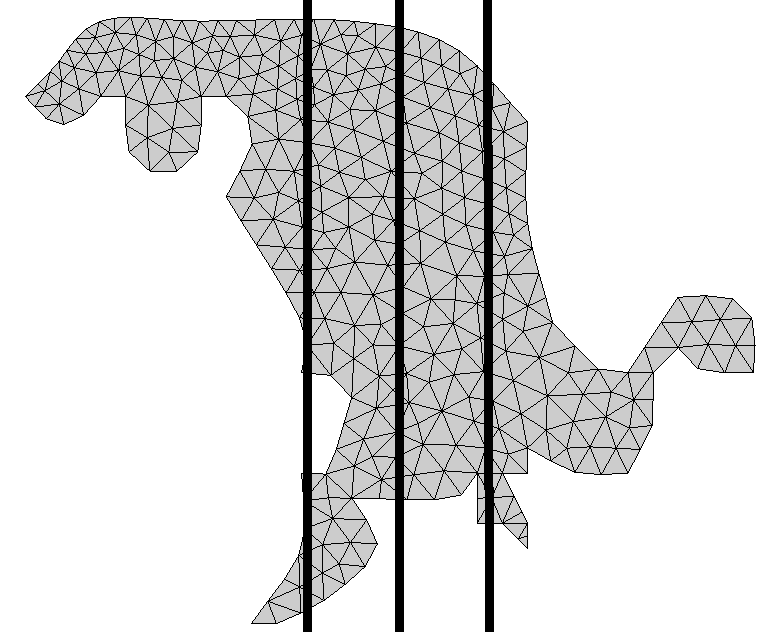
\includegraphics[width=\columnwidth]{foz_p4_msh}
		\caption{4 partitions}
		\label{fig:foz_p4_msh}
	\end{subfigure}%

	\caption{Mesh partitioning illustration}
	\label{fig:partitioning}
\end{figure}

With this partitioning method, communication is also greatly simplified, as it is guaranteed that every partition will have a left and a right neighbor. It is also assumed that the width of the global mesh is big enough so that there are never processes with 0 cells assigned, which would break communication. Since a common mesh usually contains at least thousands of cells, this should not be an issue.
On the other hand, the partitioning and assignement of the cells is done sequentially, and will increase preparation time.

\subsection{Communication Analysis}
\label{subsec:mpi:comm}

When computing the flux for a given edge, the pollution values of both adjacent cells are required. Until now, only one divergent case existed, when the edge was in the border of the mesh. With the addition of partitioning, a new divergence is created, when the edge is not in the border of the global mesh, but in the border of the local partition, meaning that one of its adjacent cells was assigned to a different partition.

A communication step is required at this point, so that each edge in the local border (the border that connects to another partition, not the global mesh border) receives the corresponding values from the neighbor partition 

This communication step was introduced at the beginning of the main loop, and consists of two smaller steps, one for left communication, and one for right communication.
Each iteration, every process starts by communicating the left border values, which were previously indexed in the preparation stage, to its left neighbor. Asynchronously with that task, it receives an equivalent message from the right neighbor, which is also at the same step. After both tasks, the direction of communication is reversed, and the right border values are sent to the right neighbor of each partition.

Only after all communication is done for this process can it continue to the main kernels of the loop. This introduces a large overhead, as it will most likely require a network transfer if the neighbor partition is located in a different machine. This overhead may become a huge bottleneck for the loop, especially for smaller inputs, where the time spent in the kernels is small enough to make the partitioning and communication occupy a large percentage of the program.

An alternative could consist in making the communication an asynchronous task, allowing the flux for inner edges to be computed while the communication is taking place, since they don't depend on the values to be received. Again, due to time constraints, it was not possible to better analyse this solution.

\subsection{Load Balance}
\label{subsec:mpi:load}

\todorev{Last revised on Sat, June 30 at 23:15 by pfac}

With the naive partitioning strategy used, load balance becomes a problem.
The computation itself is actually well balanced, since it is assured that every partition has the same amount of cells (differing at most by one). The problem is in the border between those partitions.
With the division by the horizontal coordinate being used, it becomes obvious that the size of the border between partitions becomes extremely dependant on the format of the mesh itself.
Other approaches, already mentioned in \cref{subsubsec:mpi:partitioning:research} attempt to deal with this, and produce partitions that minimize the size of the border.

The drawback of not controlling border sizes comes at the communication step.
Not only a different partitioning solution could minimize the border, thus minimizing the amount of data transfered, it can also happen that different partitions have very different border sizes, compromising communication balance.

\todonaps{Anhe? Esta última frase faz grande sentido para mim.}


\section{CUDA Implementation}
\label{sec:600}

\todosec{CUDA implementation}
Part of the work of this project was to study the parallelization methods and issues of finite volume schemes in a massively parallel architecture, specifically a GPU, using CUDA as the development technology. Some considerations can be made about the parallelization of each of the schemes presented.

The first-order scheme is the simpler one, with each value of the solution at the end of each iteration being computed based only on the strictly adjacent elements of the mesh. As a result, it should come as no surprise that it was also the one that showed better performance. The higher locality gained from only using adjacent values for each edge allows for much greater locality and less memory overhead than the second-order counterparts.

As for the second-order schemes, before any actual measurements were done, it was expected that the MUSCL would provide a greater occupancy of the GPU, which does not necessarily mean its execution time would be better. The MOOD method spends a significant portion of its time fixing errors on the detected cells. Since these cells usually represent a very small percentage of the entire domain, this means that most of the computational units will be idle, or doing useless work. In MUSCL, this is not the case, as for every interface there is a strict process of building the initial reconstruction, computing the $\Phi$ limiter for that interface, and then limit the reconstruction.
>>>>>>> aea760d4c8dcdaf00e10c898f26cd1585b078d13

\section{Experiment}
\subsection{Environmental Setup}
\todo[inline]{Describe the hex nodes}
\todo[inline]{Add a roofline for each type of nodes described}
\todo[inline]{Calculate Amdahl's Law for each hardware group}
\todo[inline]{No problem in sending this to an appendix -> and it should}
\subsection{Methodology}
\todo[inline]{Explain the hows and whys of the latest methodology}
\todo[inline]{Add the methodologies from all the phases which were not retested}
\todo[inline]{No problem in sending this to an appendix -> and it should}
\subsection{Results}
\todo[inline]{Only describe the results, a.k.a. translate every chart to words}
\subsection{Analysis}
\todo[inline]{Interpret every chart. Say what each means, what can be concluded from it}
\todo[inline]{Merge this subsection with the results if time is of the essence}

\section{Conclusion}
\todo[inline]{Sum all this shit up.}
\todo[inline,color=green!40]{Or in my own words: Sum the fuck out of this shit}











% An example of a floating figure using the graphicx package.
% Note that \label must occur AFTER (or within) \caption.
% For figures, \caption should occur after the \includegraphics.
% Note that IEEEtran v1.7 and later has special internal code that
% is designed to preserve the operation of \label within \caption
% even when the captionsoff option is in effect. However, because
% of issues like this, it may be the safest practice to put all your
% \label just after \caption rather than within \caption{}.
%
% Reminder: the "draftcls" or "draftclsnofoot", not "draft", class
% option should be used if it is desired that the figures are to be
% displayed while in draft mode.
%
%\begin{figure}[!t]
%\centering
%\includegraphics[width=2.5in]{myfigure}
% where an .eps filename suffix will be assumed under latex, 
% and a .pdf suffix will be assumed for pdflatex; or what has been declared
% via \DeclareGraphicsExtensions.
%\caption{Simulation Results}
%\label{fig_sim}
%\end{figure}

% Note that IEEE typically puts floats only at the top, even when this
% results in a large percentage of a column being occupied by floats.
% However, the Computer Society has been known to put floats at the bottom.


% An example of a double column floating figure using two subfigures.
% (The subfig.sty package must be loaded for this to work.)
% The subfigure \label commands are set within each subfloat command, the
% \label for the overall figure must come after \caption.
% \hfil must be used as a separator to get equal spacing.
% The subfigure.sty package works much the same way, except \subfigure is
% used instead of \subfloat.
%
%\begin{figure*}[!t]
%\centerline{\subfloat[Case I]\includegraphics[width=2.5in]{subfigcase1}%
%\label{fig_first_case}}
%\hfil
%\subfloat[Case II]{\includegraphics[width=2.5in]{subfigcase2}%
%\label{fig_second_case}}}
%\caption{Simulation results}
%\label{fig_sim}
%\end{figure*}
%
% Note that often IEEE papers with subfigures do not employ subfigure
% captions (using the optional argument to \subfloat), but instead will
% reference/describe all of them (a), (b), etc., within the main caption.


% An example of a floating table. Note that, for IEEE style tables, the 
% \caption command should come BEFORE the table. Table text will default to
% \footnotesize as IEEE normally uses this smaller font for tables.
% The \label must come after \caption as always.
%
%\begin{table}[!t]
%% increase table row spacing, adjust to taste
%\renewcommand{\arraystretch}{1.3}
% if using array.sty, it might be a good idea to tweak the value of
% \extrarowheight as needed to properly center the text within the cells
%\caption{An Example of a Table}
%\label{table_example}
%\centering
%% Some packages, such as MDW tools, offer better commands for making tables
%% than the plain LaTeX2e tabular which is used here.
%\begin{tabular}{|c||c|}
%\hline
%One & Two\\
%\hline
%Three & Four\\
%\hline
%\end{tabular}
%\end{table}


% Note that IEEE does not put floats in the very first column - or typically
% anywhere on the first page for that matter. Also, in-text middle ("here")
% positioning is not used. Most IEEE journals use top floats exclusively.
% However, Computer Society journals sometimes do use bottom floats - bear
% this in mind when choosing appropriate optional arguments for the
% figure/table environments.
% Note that, LaTeX2e, unlike IEEE journals, places footnotes above bottom
% floats. This can be corrected via the \fnbelowfloat command of the
% stfloats package.



% \section{Conclusion}
% The conclusion goes here.





% if have a single appendix:
%\appendix[Proof of the Zonklar Equations]
% or
%\appendix  % for no appendix heading
% do not use \section anymore after \appendix, only \section*
% is possibly needed

% use appendices with more than one appendix
% then use \section to start each appendix
% you must declare a \section before using any
% \subsection or using \label (\appendices by itself
% starts a section numbered zero.)
%


\appendices
% \section{Proof of the First Zonklar Equation}
% Appendix one text goes here.

% you can choose not to have a title for an appendix
% if you want by leaving the argument blank
% \section{}
% Appendix two text goes here.


% use section* for acknowledgement
% \ifCLASSOPTIONcompsoc
%   % The Computer Society usually uses the plural form
%   \section*{Acknowledgments}
% \else
%   % regular IEEE prefers the singular form
%   \section*{Acknowledgment}
% \fi


% The authors would like to thank...


% Can use something like this to put references on a page
% by themselves when using endfloat and the captionsoff option.
% \ifCLASSOPTIONcaptionsoff
%   \newpage
% \fi



% trigger a \newpage just before the given reference
% number - used to balance the columns on the last page
% adjust value as needed - may need to be readjusted if
% the document is modified later
%\IEEEtriggeratref{8}
% The "triggered" command can be changed if desired:
%\IEEEtriggercmd{\enlargethispage{-5in}}

% references section

% can use a bibliography generated by BibTeX as a .bbl file
% BibTeX documentation can be easily obtained at:
% http://www.ctan.org/tex-archive/biblio/bibtex/contrib/doc/
% The IEEEtran BibTeX style support page is at:
% http://www.michaelshell.org/tex/ieeetran/bibtex/
\bibliographystyle{IEEEtran}
% % argument is your BibTeX string definitions and bibliography database(s)
%\bibliography{../IEEE/IEEEabrv,../references}
\bibliography{../references}
%
% <OR> manually copy in the resultant .bbl file
% set second argument of \begin to the number of references
% (used to reserve space for the reference number labels box)
%\begin{thebibliography}{1}

%\bibitem{IEEEhowto:kopka}
%H.~Kopka and P.~W. Daly, \emph{A Guide to \LaTeX}, 3rd~ed.\hskip 1em plus
%  0.5em minus 0.4em\relax Harlow, England: Addison-Wesley, 1999.

%\end{thebibliography}

% biography section
% 
% If you have an EPS/PDF photo (graphicx package needed) extra braces are
% needed around the contents of the optional argument to biography to prevent
% the LaTeX parser from getting confused when it sees the complicated
% \includegraphics command within an optional argument. (You could create
% your own custom macro containing the \includegraphics command to make things
% simpler here.)
%\begin{biography}[{\includegraphics[width=1in,height=1.25in,clip,keepaspectratio]{mshell}}]{Michael Shell}
% or if you just want to reserve a space for a photo:

% \begin{IEEEbiography}{Michael Shell}
% Biography text here.
% \end{IEEEbiography}

% if you will not have a photo at all:
% \begin{IEEEbiographynophoto}{John Doe}
% Biography text here.
% \end{IEEEbiographynophoto}

% insert where needed to balance the two columns on the last page with
% biographies
%\newpage

% \begin{IEEEbiographynophoto}{Jane Doe}
% Biography text here.
% \end{IEEEbiographynophoto}

% You can push biographies down or up by placing
% a \vfill before or after them. The appropriate
% use of \vfill depends on what kind of text is
% on the last page and whether or not the columns
% are being equalized.

%\vfill

% Can be used to pull up biographies so that the bottom of the last one
% is flush with the other column.
%\enlargethispage{-5in}



% that's all folks
\end{document}


